\documentclass{article}

\usepackage{noweb}
\noweboptions{smallcode,longchunks}
\usepackage[a4paper,margin=1in]{geometry}
\usepackage{colortbl}
\usepackage[colorlinks=true]{hyperref}
\usepackage{tikz}

\newcommand{\hi}[1]{\noindent {\bf #1}}     % Define a handy paragraph opener

\def\nwendcode{\endtrivlist \endgroup}      % Remove noweb page break penalty
\let\nwdocspar=\par

\title{Jargo Client\footnote{
    \url{https://github.com/jargors/Client}}}
\author{James J. Pan\\
  \small{\href{mailto:pan-j16@mails.tsinghua.edu.cn}{pan-j16@mails.tsinghua.edu.cn}}}

\begin{document}
\maketitle
\pagestyle{noweb}

\tableofcontents

\section{Introduction}
\label{sec:introduction}
We supply an abstract base class for developing Jargo client ridesharing
algorithms. The class provides a standard interface for interacting with the
simulation engine (Figure~\ref{fig:client}). Algorithm developers extend the
base class to add specific customer-to-vehicle matching and vehicle routing
functionality.  The base class is developed using the
Noweb\footnote{\url{https://www.cs.tufts.edu/~nr/noweb/}} literate
programming\footnote{\url{http://literateprogramming.com/}} tool.  This file
({\tt{}src/Client.nw}) is the source for both the documentation
({\tt{}doc/Client.tex}) and the Java code (Client.java)\footnote{See the
{\tt{}Makefile} for build details.}.

\begin{figure}[h]
\centering
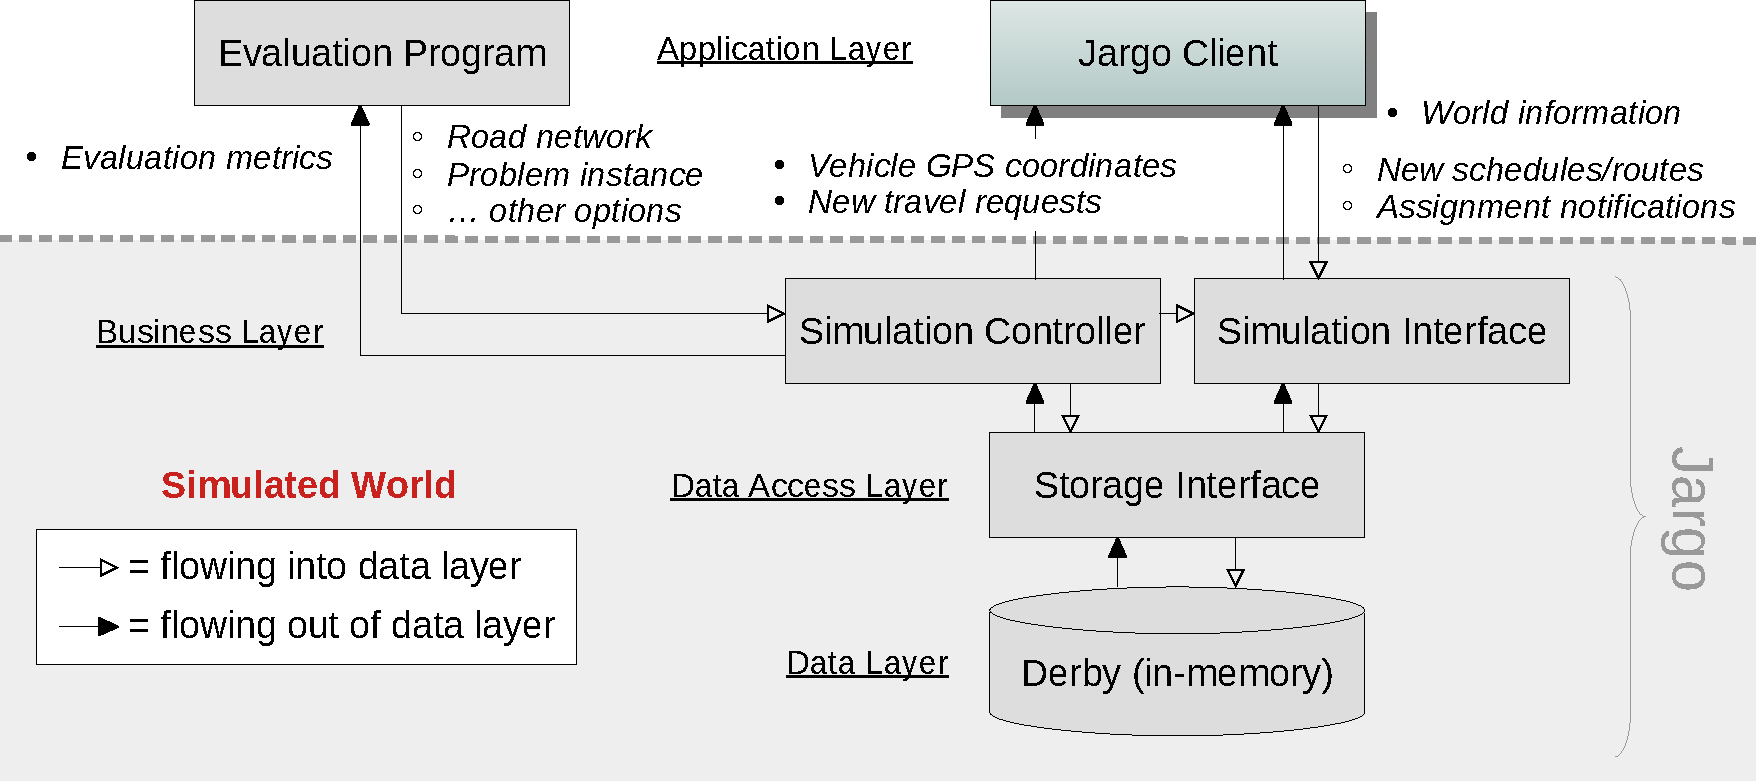
\includegraphics[width=150mm]{src/fig/client-fig}
\caption{Client within the Jargo stack.}
\label{fig:client}
\end{figure}

\section{Implementation Overview}
\nwfilename{src/Client.nw}\nwbegincode{1}\sublabel{NW2q3QGT-bpC9O-1}\nwmargintag{{\nwtagstyle{}\subpageref{NW2q3QGT-bpC9O-1}}}\moddef{Client.java~{\nwtagstyle{}\subpageref{NW2q3QGT-bpC9O-1}}}\endmoddef\nwnotused{Client.java}
\LA{}Client.java preamble~{\nwtagstyle{}\subpageref{NW2q3QGT-xBgX1-1}}\RA{}
\LA{}\code{}Client\edoc{} definition~{\nwtagstyle{}\subpageref{NW2q3QGT-3hr6Rs-1}}\RA{}
\nwendcode{}\nwbegindocs{2}\nwdocspar

\subsection{Preamble}
The preamble declares the package and imports dependencies.
\nwenddocs{}\nwbegincode{3}\sublabel{NW2q3QGT-xBgX1-1}\nwmargintag{{\nwtagstyle{}\subpageref{NW2q3QGT-xBgX1-1}}}\moddef{Client.java preamble~{\nwtagstyle{}\subpageref{NW2q3QGT-xBgX1-1}}}\endmoddef\nwalsodefined{\\{NW2q3QGT-xBgX1-2}}\nwused{\\{NW2q3QGT-bpC9O-1}}
package com.github.jargors;
\nwendcode{}\nwbegindocs{4}\nwdocspar
We import {\tt{}Communicator} so we can interact with the simulated world,
and we import {\tt{}LocalDateTime} so we can query the physical time for
logging purposes.
\nwenddocs{}\nwbegincode{5}\sublabel{NW2q3QGT-xBgX1-2}\nwmargintag{{\nwtagstyle{}\subpageref{NW2q3QGT-xBgX1-2}}}\moddef{Client.java preamble~{\nwtagstyle{}\subpageref{NW2q3QGT-xBgX1-1}}}\plusendmoddef
import com.github.jargors.Communicator;
import com.github.jargors.Tools;
import java.util.function.Supplier;
import java.util.concurrent.ConcurrentLinkedQueue;
import java.time.LocalDateTime;
\nwendcode{}\nwbegindocs{6}\nwdocspar

\subsection{Class Definition}
The {\tt{}Client} class consists of member variables, a constructor, and
public and protected methods. Note the {\tt{}abstract} keyword indicates the class
cannot be used directly.
\nwenddocs{}\nwbegincode{7}\sublabel{NW2q3QGT-3hr6Rs-1}\nwmargintag{{\nwtagstyle{}\subpageref{NW2q3QGT-3hr6Rs-1}}}\moddef{\code{}Client\edoc{} definition~{\nwtagstyle{}\subpageref{NW2q3QGT-3hr6Rs-1}}}\endmoddef\nwused{\\{NW2q3QGT-bpC9O-1}}
public abstract class Client \{
  \LA{}\code{}Client\edoc{} member variables~{\nwtagstyle{}\subpageref{NW2q3QGT-3qCSiR-1}}\RA{}
  \LA{}\code{}Client\edoc{} constructor~{\nwtagstyle{}\subpageref{NW2q3QGT-2crckK-1}}\RA{}
  \LA{}\code{}Client\edoc{} public methods~{\nwtagstyle{}\subpageref{NW2q3QGT-4VlNed-1}}\RA{}
  \LA{}\code{}Client\edoc{} protected methods~{\nwtagstyle{}\subpageref{NW2q3QGT-4EUu6m-1}}\RA{}
\}
\nwendcode{}\nwbegindocs{8}\nwdocspar

\subsection{Member Variables}
\nwenddocs{}\nwbegincode{9}\sublabel{NW2q3QGT-3qCSiR-1}\nwmargintag{{\nwtagstyle{}\subpageref{NW2q3QGT-3qCSiR-1}}}\moddef{\code{}Client\edoc{} member variables~{\nwtagstyle{}\subpageref{NW2q3QGT-3qCSiR-1}}}\endmoddef\nwused{\\{NW2q3QGT-3hr6Rs-1}}
protected ConcurrentLinkedQueue<int[]> queue = new ConcurrentLinkedQueue();
protected int r_collection_period = 1;  // how many sec before collecting new req?
protected int r_handling_period = 1;  // how many msec before handling queued req?
protected int s_collection_period = 10;
protected Communicator communicator;
protected Tools tools = new Tools();
protected boolean DEBUG = false;
\nwindexdefn{queue}{queue}{NW2q3QGT-3qCSiR-1}\nwindexdefn{r{\char95}collection{\char95}period}{r:uncollection:unperiod}{NW2q3QGT-3qCSiR-1}\nwindexdefn{r{\char95}handling{\char95}period}{r:unhandling:unperiod}{NW2q3QGT-3qCSiR-1}\nwindexdefn{s{\char95}collection{\char95}period}{s:uncollection:unperiod}{NW2q3QGT-3qCSiR-1}\nwindexdefn{communicator}{communicator}{NW2q3QGT-3qCSiR-1}\nwindexdefn{tools}{tools}{NW2q3QGT-3qCSiR-1}\nwindexdefn{DEBUG}{DEBUG}{NW2q3QGT-3qCSiR-1}\eatline
\nwidentdefs{\\{{communicator}{communicator}}\\{{DEBUG}{DEBUG}}\\{{queue}{queue}}\\{{r{\char95}collection{\char95}period}{r:uncollection:unperiod}}\\{{r{\char95}handling{\char95}period}{r:unhandling:unperiod}}\\{{s{\char95}collection{\char95}period}{s:uncollection:unperiod}}\\{{tools}{tools}}}\nwendcode{}\nwbegindocs{10}\nwdocspar
\subsection{Constructor}
\nwenddocs{}\nwbegincode{11}\sublabel{NW2q3QGT-2crckK-1}\nwmargintag{{\nwtagstyle{}\subpageref{NW2q3QGT-2crckK-1}}}\moddef{\code{}Client\edoc{} constructor~{\nwtagstyle{}\subpageref{NW2q3QGT-2crckK-1}}}\endmoddef\nwused{\\{NW2q3QGT-3hr6Rs-1}}
public Client() \{ \}
\nwendcode{}\nwbegindocs{12}\nwdocspar

\section{Public Methods}
\nwenddocs{}\nwbegincode{13}\sublabel{NW2q3QGT-4VlNed-1}\nwmargintag{{\nwtagstyle{}\subpageref{NW2q3QGT-4VlNed-1}}}\moddef{\code{}Client\edoc{} public methods~{\nwtagstyle{}\subpageref{NW2q3QGT-4VlNed-1}}}\endmoddef\nwused{\\{NW2q3QGT-3hr6Rs-1}}
  \LA{}Notify new requests~{\nwtagstyle{}\subpageref{NW2q3QGT-38hTAx-1}}\RA{}
  \LA{}Collect request into queue~{\nwtagstyle{}\subpageref{NW2q3QGT-2IDYop-1}}\RA{}
  \LA{}Collect server locations~{\nwtagstyle{}\subpageref{NW2q3QGT-wbUkp-1}}\RA{}
  \LA{}Set simulation interface~{\nwtagstyle{}\subpageref{NW2q3QGT-4etKpU-1}}\RA{}
  \LA{}Set debug flag~{\nwtagstyle{}\subpageref{NW2q3QGT-2DhHFw-1}}\RA{}
  \LA{}Get/set request collection period~{\nwtagstyle{}\subpageref{NW2q3QGT-4fmrsw-1}}\RA{}
  \LA{}Get/set request handling period~{\nwtagstyle{}\subpageref{NW2q3QGT-3bGa5x-1}}\RA{}
  \LA{}Get/set server location collection period~{\nwtagstyle{}\subpageref{NW2q3QGT-DxGq5-1}}\RA{}
  \LA{}Load GTree~{\nwtagstyle{}\subpageref{NW2q3QGT-b7Jka-1}}\RA{}
  \LA{}Register road network~{\nwtagstyle{}\subpageref{NW2q3QGT-3hO9hR-1}}\RA{}
  \LA{}Register users~{\nwtagstyle{}\subpageref{NW2q3QGT-UKHEr-1}}\RA{}
\nwendcode{}\nwbegindocs{14}\nwdocspar

\subsection{Obtaining Requests and Server Locations}

\subsubsection{{\tt{}\protect\nosublabel{NW2q3QGT-4VlNed-1-u11}\protect\nwindexuse{notifyNew}{notifyNew}{NW2q3QGT-38hTAx-1}notifyNew}(0)}
\nwenddocs{}\nwbegincode{15}\sublabel{NW2q3QGT-38hTAx-1}\nwmargintag{{\nwtagstyle{}\subpageref{NW2q3QGT-38hTAx-1}}}\moddef{Notify new requests~{\nwtagstyle{}\subpageref{NW2q3QGT-38hTAx-1}}}\endmoddef\nwused{\\{NW2q3QGT-4VlNed-1}}
public void notifyNew() \{
  if (!queue.isEmpty()) \{
    handleRequest(queue.remove());
  \}
\}
\nwindexdefn{notifyNew}{notifyNew}{NW2q3QGT-38hTAx-1}\eatline
\nwidentdefs{\\{{notifyNew}{notifyNew}}}\nwidentuses{\\{{handleRequest}{handleRequest}}\\{{queue}{queue}}}\nwindexuse{handleRequest}{handleRequest}{NW2q3QGT-38hTAx-1}\nwindexuse{queue}{queue}{NW2q3QGT-38hTAx-1}\nwendcode{}\nwbegindocs{16}\nwdocspar
\subsubsection{{\tt{}collectRequest}(1)}
\nwenddocs{}\nwbegincode{17}\sublabel{NW2q3QGT-2IDYop-1}\nwmargintag{{\nwtagstyle{}\subpageref{NW2q3QGT-2IDYop-1}}}\moddef{Collect request into queue~{\nwtagstyle{}\subpageref{NW2q3QGT-2IDYop-1}}}\endmoddef\nwused{\\{NW2q3QGT-4VlNed-1}}
public void collectRequest(int[] r) \{
  queue.add(r);
\}
\nwindexdefn{addRequest}{addRequest}{NW2q3QGT-2IDYop-1}\eatline
\nwidentdefs{\\{{addRequest}{addRequest}}}\nwidentuses{\\{{queue}{queue}}}\nwindexuse{queue}{queue}{NW2q3QGT-2IDYop-1}\nwendcode{}\nwbegindocs{18}\nwdocspar
\subsubsection{{\tt{}\protect\nwindexuse{collectServerLocations}{collectServerLocations}{NW2q3QGT-wbUkp-1}collectServerLocations}(1)}
Array {\tt{}src} =

\noindent
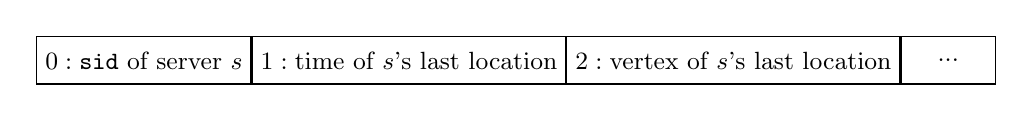
\begin{tikzpicture}
\small
\matrix[nodes={draw,minimum size=6mm}] {
  \node {$0:\textrm{{\tt{}sid} of server }s$};
 &\node {$1:\textrm{time of $s$'s last location}$};
 &\node {$2:\textrm{vertex of $s$'s last location}$};
 &\node[minimum width=12mm] {...};\\
};
\end{tikzpicture}

\noindent If locations are polled for and stored into {\tt{}src} at $t'$ world
time, then formally the last location for server $s$ is defined as waypoint
$(t,v)$ that satisfies $t=\textrm{argmin}_{(t,v)\in w_{\leq t'}} (t-t')$, where
$w_{\leq t'}$ is the server's traveled route.  In other words the last location
is the waypoint in the server's traveled route that is nearest $t'$.  After
copying {\tt{}src} into {\tt{}locations}, the {\tt{}\protect\nwindexuse{endCollectServerLocations}{endCollectServerLocations}{NW2q3QGT-2d6rGZ-1}endCollectServerLocations}(0) method
is executed.
\nwenddocs{}\nwbegincode{19}\sublabel{NW2q3QGT-wbUkp-1}\nwmargintag{{\nwtagstyle{}\subpageref{NW2q3QGT-wbUkp-1}}}\moddef{Collect server locations~{\nwtagstyle{}\subpageref{NW2q3QGT-wbUkp-1}}}\endmoddef\nwused{\\{NW2q3QGT-4VlNed-1}}
public void collectServerLocations(int[] src) \{
  int[] locations = src.clone();
  endCollectServerLocations(locations);
\}
\nwindexdefn{collectServerLocations}{collectServerLocations}{NW2q3QGT-wbUkp-1}\eatline
\nwidentdefs{\\{{collectServerLocations}{collectServerLocations}}}\nwidentuses{\\{{endCollectServerLocations}{endCollectServerLocations}}}\nwindexuse{endCollectServerLocations}{endCollectServerLocations}{NW2q3QGT-wbUkp-1}\nwendcode{}\nwbegindocs{20}\nwdocspar
\subsection{Getters and Setters}

\subsubsection{{\tt{}\protect\nwindexuse{setCommunicator}{setCommunicator}{NW2q3QGT-4etKpU-1}setCommunicator}(1)}
\nwenddocs{}\nwbegincode{21}\sublabel{NW2q3QGT-4etKpU-1}\nwmargintag{{\nwtagstyle{}\subpageref{NW2q3QGT-4etKpU-1}}}\moddef{Set simulation interface~{\nwtagstyle{}\subpageref{NW2q3QGT-4etKpU-1}}}\endmoddef\nwused{\\{NW2q3QGT-4VlNed-1}}
public void setCommunicator(Communicator src) \{
  communicator = src;
\}
\nwindexdefn{setCommunicator}{setCommunicator}{NW2q3QGT-4etKpU-1}\eatline
\nwidentdefs{\\{{setCommunicator}{setCommunicator}}}\nwidentuses{\\{{communicator}{communicator}}}\nwindexuse{communicator}{communicator}{NW2q3QGT-4etKpU-1}\nwendcode{}\nwbegindocs{22}\nwdocspar
\subsubsection{{\tt{}\protect\nwindexuse{setDebug}{setDebug}{NW2q3QGT-2DhHFw-1}setDebug}(1)}
\nwenddocs{}\nwbegincode{23}\sublabel{NW2q3QGT-2DhHFw-1}\nwmargintag{{\nwtagstyle{}\subpageref{NW2q3QGT-2DhHFw-1}}}\moddef{Set debug flag~{\nwtagstyle{}\subpageref{NW2q3QGT-2DhHFw-1}}}\endmoddef\nwused{\\{NW2q3QGT-4VlNed-1}}
public void setDebug(boolean flag) \{
  DEBUG = flag;
\}
\nwindexdefn{setDebug}{setDebug}{NW2q3QGT-2DhHFw-1}\eatline
\nwidentdefs{\\{{setDebug}{setDebug}}}\nwidentuses{\\{{DEBUG}{DEBUG}}}\nwindexuse{DEBUG}{DEBUG}{NW2q3QGT-2DhHFw-1}\nwendcode{}\nwbegindocs{24}\nwdocspar
\subsubsection{{\tt{}\protect\nwindexuse{getRequestCollectionPeriod}{getRequestCollectionPeriod}{NW2q3QGT-4fmrsw-1}getRequestCollectionPeriod}(0)}
\nwenddocs{}\nwbegincode{25}\sublabel{NW2q3QGT-4fmrsw-1}\nwmargintag{{\nwtagstyle{}\subpageref{NW2q3QGT-4fmrsw-1}}}\moddef{Get/set request collection period~{\nwtagstyle{}\subpageref{NW2q3QGT-4fmrsw-1}}}\endmoddef\nwalsodefined{\\{NW2q3QGT-4fmrsw-2}}\nwused{\\{NW2q3QGT-4VlNed-1}}
public int getRequestCollectionPeriod() \{
  return r_collection_period;
\}
\nwindexdefn{getRequestCollectionPeriod}{getRequestCollectionPeriod}{NW2q3QGT-4fmrsw-1}\eatline
\nwidentdefs{\\{{getRequestCollectionPeriod}{getRequestCollectionPeriod}}}\nwidentuses{\\{{r{\char95}collection{\char95}period}{r:uncollection:unperiod}}}\nwindexuse{r{\char95}collection{\char95}period}{r:uncollection:unperiod}{NW2q3QGT-4fmrsw-1}\nwendcode{}\nwbegindocs{26}\nwdocspar
\subsubsection{{\tt{}\protect\nwindexuse{setRequestCollectionPeriod}{setRequestCollectionPeriod}{NW2q3QGT-4fmrsw-2}setRequestCollectionPeriod}(1)}
\nwenddocs{}\nwbegincode{27}\sublabel{NW2q3QGT-4fmrsw-2}\nwmargintag{{\nwtagstyle{}\subpageref{NW2q3QGT-4fmrsw-2}}}\moddef{Get/set request collection period~{\nwtagstyle{}\subpageref{NW2q3QGT-4fmrsw-1}}}\plusendmoddef
public void setRequestCollectionPeriod(int t) \{
  r_collection_period = t;
\}
\nwindexdefn{setRequestCollectionPeriod}{setRequestCollectionPeriod}{NW2q3QGT-4fmrsw-2}\eatline
\nwidentdefs{\\{{setRequestCollectionPeriod}{setRequestCollectionPeriod}}}\nwidentuses{\\{{r{\char95}collection{\char95}period}{r:uncollection:unperiod}}}\nwindexuse{r{\char95}collection{\char95}period}{r:uncollection:unperiod}{NW2q3QGT-4fmrsw-2}\nwendcode{}\nwbegindocs{28}\nwdocspar
\subsubsection{{\tt{}\protect\nwindexuse{getRequestHandlingPeriod}{getRequestHandlingPeriod}{NW2q3QGT-3bGa5x-1}getRequestHandlingPeriod}(1)}
\nwenddocs{}\nwbegincode{29}\sublabel{NW2q3QGT-3bGa5x-1}\nwmargintag{{\nwtagstyle{}\subpageref{NW2q3QGT-3bGa5x-1}}}\moddef{Get/set request handling period~{\nwtagstyle{}\subpageref{NW2q3QGT-3bGa5x-1}}}\endmoddef\nwalsodefined{\\{NW2q3QGT-3bGa5x-2}}\nwused{\\{NW2q3QGT-4VlNed-1}}
public int getRequestHandlingPeriod() \{
  return r_handling_period;
\}
\nwindexdefn{getRequestHandlingPeriod}{getRequestHandlingPeriod}{NW2q3QGT-3bGa5x-1}\eatline
\nwidentdefs{\\{{getRequestHandlingPeriod}{getRequestHandlingPeriod}}}\nwidentuses{\\{{r{\char95}handling{\char95}period}{r:unhandling:unperiod}}}\nwindexuse{r{\char95}handling{\char95}period}{r:unhandling:unperiod}{NW2q3QGT-3bGa5x-1}\nwendcode{}\nwbegindocs{30}\nwdocspar
\subsubsection{{\tt{}\protect\nwindexuse{setRequestHandlingPeriod}{setRequestHandlingPeriod}{NW2q3QGT-3bGa5x-2}setRequestHandlingPeriod}(0)}
\nwenddocs{}\nwbegincode{31}\sublabel{NW2q3QGT-3bGa5x-2}\nwmargintag{{\nwtagstyle{}\subpageref{NW2q3QGT-3bGa5x-2}}}\moddef{Get/set request handling period~{\nwtagstyle{}\subpageref{NW2q3QGT-3bGa5x-1}}}\plusendmoddef
public void setRequestHandlingPeriod(int t) \{
  r_handling_period = t;
\}
\nwindexdefn{setRequestHandlingPeriod}{setRequestHandlingPeriod}{NW2q3QGT-3bGa5x-2}\eatline
\nwidentdefs{\\{{setRequestHandlingPeriod}{setRequestHandlingPeriod}}}\nwidentuses{\\{{r{\char95}handling{\char95}period}{r:unhandling:unperiod}}}\nwindexuse{r{\char95}handling{\char95}period}{r:unhandling:unperiod}{NW2q3QGT-3bGa5x-2}\nwendcode{}\nwbegindocs{32}\nwdocspar
\subsubsection{{\tt{}\protect\nwindexuse{getServerLocationCollectionPeriod}{getServerLocationCollectionPeriod}{NW2q3QGT-DxGq5-1}getServerLocationCollectionPeriod}(0)}
\nwenddocs{}\nwbegincode{33}\sublabel{NW2q3QGT-DxGq5-1}\nwmargintag{{\nwtagstyle{}\subpageref{NW2q3QGT-DxGq5-1}}}\moddef{Get/set server location collection period~{\nwtagstyle{}\subpageref{NW2q3QGT-DxGq5-1}}}\endmoddef\nwalsodefined{\\{NW2q3QGT-DxGq5-2}}\nwused{\\{NW2q3QGT-4VlNed-1}}
public int getServerLocationCollectionPeriod () \{
  return s_collection_period;
\}
\nwindexdefn{getServerLocationCollectionPeriod}{getServerLocationCollectionPeriod}{NW2q3QGT-DxGq5-1}\eatline
\nwidentdefs{\\{{getServerLocationCollectionPeriod}{getServerLocationCollectionPeriod}}}\nwidentuses{\\{{s{\char95}collection{\char95}period}{s:uncollection:unperiod}}}\nwindexuse{s{\char95}collection{\char95}period}{s:uncollection:unperiod}{NW2q3QGT-DxGq5-1}\nwendcode{}\nwbegindocs{34}\nwdocspar
\subsubsection{{\tt{}\protect\nwindexuse{setServerLocationCollectionPeriod}{setServerLocationCollectionPeriod}{NW2q3QGT-DxGq5-2}setServerLocationCollectionPeriod}(1)}
\nwenddocs{}\nwbegincode{35}\sublabel{NW2q3QGT-DxGq5-2}\nwmargintag{{\nwtagstyle{}\subpageref{NW2q3QGT-DxGq5-2}}}\moddef{Get/set server location collection period~{\nwtagstyle{}\subpageref{NW2q3QGT-DxGq5-1}}}\plusendmoddef
public void setServerLocationCollectionPeriod(int t) \{
  s_collection_period = t;
\}
\nwindexdefn{setServerLocationCollectionPeriod}{setServerLocationCollectionPeriod}{NW2q3QGT-DxGq5-2}\eatline
\nwidentdefs{\\{{setServerLocationCollectionPeriod}{setServerLocationCollectionPeriod}}}\nwidentuses{\\{{s{\char95}collection{\char95}period}{s:uncollection:unperiod}}}\nwindexuse{s{\char95}collection{\char95}period}{s:uncollection:unperiod}{NW2q3QGT-DxGq5-2}\nwendcode{}\nwbegindocs{36}\nwdocspar
\subsubsection{{\tt{}\protect\nwindexuse{loadGTree}{loadGTree}{NW2q3QGT-b7Jka-1}loadGTree}(1)}
\nwenddocs{}\nwbegincode{37}\sublabel{NW2q3QGT-b7Jka-1}\nwmargintag{{\nwtagstyle{}\subpageref{NW2q3QGT-b7Jka-1}}}\moddef{Load GTree~{\nwtagstyle{}\subpageref{NW2q3QGT-b7Jka-1}}}\endmoddef\nwused{\\{NW2q3QGT-4VlNed-1}}
public void loadGTree(String p) \{
  tools.loadGTree(p);
\}
\nwindexdefn{loadGTree}{loadGTree}{NW2q3QGT-b7Jka-1}\eatline
\nwidentdefs{\\{{loadGTree}{loadGTree}}}\nwidentuses{\\{{tools}{tools}}}\nwindexuse{tools}{tools}{NW2q3QGT-b7Jka-1}\nwendcode{}\nwbegindocs{38}\nwdocspar
\subsubsection{{\tt{}\protect\nwindexuse{registerRoadNetwork}{registerRoadNetwork}{NW2q3QGT-3hO9hR-1}registerRoadNetwork}(0)}
\nwenddocs{}\nwbegincode{39}\sublabel{NW2q3QGT-3hO9hR-1}\nwmargintag{{\nwtagstyle{}\subpageref{NW2q3QGT-3hO9hR-1}}}\moddef{Register road network~{\nwtagstyle{}\subpageref{NW2q3QGT-3hO9hR-1}}}\endmoddef\nwused{\\{NW2q3QGT-4VlNed-1}}
public void registerRoadNetwork() \{
  tools.registerVertices(communicator.getReferenceVerticesCache());
  tools.registerEdges(communicator.getReferenceEdgesCache());
\}
\nwindexdefn{registerRoadNetwork}{registerRoadNetwork}{NW2q3QGT-3hO9hR-1}\eatline
\nwidentdefs{\\{{registerRoadNetwork}{registerRoadNetwork}}}\nwidentuses{\\{{communicator}{communicator}}\\{{tools}{tools}}}\nwindexuse{communicator}{communicator}{NW2q3QGT-3hO9hR-1}\nwindexuse{tools}{tools}{NW2q3QGT-3hO9hR-1}\nwendcode{}\nwbegindocs{40}\nwdocspar
\subsubsection{{\tt{}\protect\nwindexuse{registerUsers}{registerUsers}{NW2q3QGT-UKHEr-1}registerUsers}(0)}
\nwenddocs{}\nwbegincode{41}\sublabel{NW2q3QGT-UKHEr-1}\nwmargintag{{\nwtagstyle{}\subpageref{NW2q3QGT-UKHEr-1}}}\moddef{Register users~{\nwtagstyle{}\subpageref{NW2q3QGT-UKHEr-1}}}\endmoddef\nwused{\\{NW2q3QGT-4VlNed-1}}
public void registerUsers() \{
  tools.registerUsers(communicator.getReferenceUsersCache());
\}
\nwindexdefn{registerUsers}{registerUsers}{NW2q3QGT-UKHEr-1}\eatline
\nwidentdefs{\\{{registerUsers}{registerUsers}}}\nwidentuses{\\{{communicator}{communicator}}\\{{tools}{tools}}}\nwindexuse{communicator}{communicator}{NW2q3QGT-UKHEr-1}\nwindexuse{tools}{tools}{NW2q3QGT-UKHEr-1}\nwendcode{}\nwbegindocs{42}\nwdocspar
\section{Private Methods}
\nwenddocs{}\nwbegincode{43}\sublabel{NW2q3QGT-4EUu6m-1}\nwmargintag{{\nwtagstyle{}\subpageref{NW2q3QGT-4EUu6m-1}}}\moddef{\code{}Client\edoc{} protected methods~{\nwtagstyle{}\subpageref{NW2q3QGT-4EUu6m-1}}}\endmoddef\nwused{\\{NW2q3QGT-3hr6Rs-1}}
  \LA{}End collect server locations~{\nwtagstyle{}\subpageref{NW2q3QGT-2d6rGZ-1}}\RA{}
  \LA{}End simulation~{\nwtagstyle{}\subpageref{NW2q3QGT-3OCf0y-1}}\RA{}
  \LA{}Handle request~{\nwtagstyle{}\subpageref{NW2q3QGT-2856ar-1}}\RA{}
  \LA{}Handle server location~{\nwtagstyle{}\subpageref{NW2q3QGT-2xqRZA-1}}\RA{}
  \LA{}Print a message~{\nwtagstyle{}\subpageref{NW2q3QGT-2wEn3G-1}}\RA{}
\nwendcode{}\nwbegindocs{44}\nwdocspar

\subsection{{\tt{}\protect\nosublabel{NW2q3QGT-4EUu6m-1-u5}\protect\nwindexuse{endCollectServerLocations}{endCollectServerLocations}{NW2q3QGT-2d6rGZ-1}endCollectServerLocations}(0)}
After server locations are collected, {\tt{}\protect\nwindexuse{handleServerLocation}{handleServerLocation}{NW2q3QGT-2xqRZA-1}handleServerLocation}(1) is executed
on each one.
\nwenddocs{}\nwbegincode{45}\sublabel{NW2q3QGT-2d6rGZ-1}\nwmargintag{{\nwtagstyle{}\subpageref{NW2q3QGT-2d6rGZ-1}}}\moddef{End collect server locations~{\nwtagstyle{}\subpageref{NW2q3QGT-2d6rGZ-1}}}\endmoddef\nwused{\\{NW2q3QGT-4EUu6m-1}}
protected void endCollectServerLocations(int[] locations) \{
  for (int i = 0; i < (locations.length - 2); i += 3) \{
    handleServerLocation(new int[] \{
      locations[i],
      locations[(i + 1)],
      locations[(i + 2)]
    \});
  \}
\}
\nwindexdefn{endCollectServerLocations}{endCollectServerLocations}{NW2q3QGT-2d6rGZ-1}\eatline
\nwidentdefs{\\{{endCollectServerLocations}{endCollectServerLocations}}}\nwidentuses{\\{{handleServerLocation}{handleServerLocation}}}\nwindexuse{handleServerLocation}{handleServerLocation}{NW2q3QGT-2d6rGZ-1}\nwendcode{}\nwbegindocs{46}\nwdocspar
\subsection{{\tt{}\protect\nwindexuse{end}{end}{NW2q3QGT-3OCf0y-1}end}(0)}
\nwenddocs{}\nwbegincode{47}\sublabel{NW2q3QGT-3OCf0y-1}\nwmargintag{{\nwtagstyle{}\subpageref{NW2q3QGT-3OCf0y-1}}}\moddef{End simulation~{\nwtagstyle{}\subpageref{NW2q3QGT-3OCf0y-1}}}\endmoddef\nwused{\\{NW2q3QGT-4EUu6m-1}}
protected void end() \{ \}
\nwindexdefn{end}{end}{NW2q3QGT-3OCf0y-1}\eatline
\nwidentdefs{\\{{end}{end}}}\nwendcode{}\nwbegindocs{48}\nwdocspar
\subsection{{\tt{}\protect\nwindexuse{handleRequest}{handleRequest}{NW2q3QGT-2856ar-1}handleRequest}(1)}
Array {\tt{}r} =

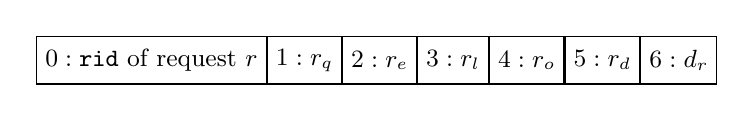
\begin{tikzpicture}
\small
\matrix[nodes={draw,minimum size=6mm}] {
  \node {$0:\textrm{{\tt{}rid} of request $r$}$};
 &\node {$1:r_q$}; & \node {$2:r_e$}; & \node {$3:r_l$};
 &\node {$4:r_o$}; & \node {$5:r_d$}; & \node {$6:d_r$};\\
};
\end{tikzpicture}

\nwenddocs{}\nwbegincode{49}\sublabel{NW2q3QGT-2856ar-1}\nwmargintag{{\nwtagstyle{}\subpageref{NW2q3QGT-2856ar-1}}}\moddef{Handle request~{\nwtagstyle{}\subpageref{NW2q3QGT-2856ar-1}}}\endmoddef\nwused{\\{NW2q3QGT-4EUu6m-1}}
protected void handleRequest(int[] r) \{ \}
\nwindexdefn{handleRequest}{handleRequest}{NW2q3QGT-2856ar-1}\eatline
\nwidentdefs{\\{{handleRequest}{handleRequest}}}\nwendcode{}\nwbegindocs{50}\nwdocspar
\subsection{{\tt{}\protect\nwindexuse{handleServerLocation}{handleServerLocation}{NW2q3QGT-2xqRZA-1}handleServerLocation}(1)}
Array {\tt{}loc} =

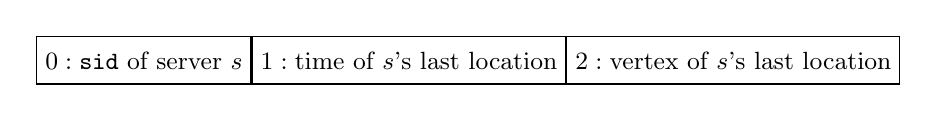
\begin{tikzpicture}
\small
\matrix[nodes={draw,minimum size=6mm}] {
  \node {$0:\textrm{{\tt{}sid} of server $s$}$};
 &\node {$1:\textrm{time of $s$'s last location}$};
 &\node {$2:\textrm{vertex of $s$'s last location}$};\\
};
\end{tikzpicture}

\nwenddocs{}\nwbegincode{51}\sublabel{NW2q3QGT-2xqRZA-1}\nwmargintag{{\nwtagstyle{}\subpageref{NW2q3QGT-2xqRZA-1}}}\moddef{Handle server location~{\nwtagstyle{}\subpageref{NW2q3QGT-2xqRZA-1}}}\endmoddef\nwused{\\{NW2q3QGT-4EUu6m-1}}
protected void handleServerLocation(int[] loc) \{ \}
\nwindexdefn{handleServerLocation}{handleServerLocation}{NW2q3QGT-2xqRZA-1}\eatline
\nwidentdefs{\\{{handleServerLocation}{handleServerLocation}}}\nwendcode{}\nwbegindocs{52}\nwdocspar
\subsection{{\tt{}\protect\nwindexuse{Print}{Print}{NW2q3QGT-2wEn3G-1}Print}(1)}
\nwenddocs{}\nwbegincode{53}\sublabel{NW2q3QGT-2wEn3G-1}\nwmargintag{{\nwtagstyle{}\subpageref{NW2q3QGT-2wEn3G-1}}}\moddef{Print a message~{\nwtagstyle{}\subpageref{NW2q3QGT-2wEn3G-1}}}\endmoddef\nwused{\\{NW2q3QGT-4EUu6m-1}}
protected void Print(String msg) \{
  if (DEBUG) \{
    System.out.println("[Client]["+LocalDateTime.now()+"]"
      + "[t="+communicator.getSimulationWorldTime()+"] "+msg);
  \}
\}
\nwindexdefn{Print}{Print}{NW2q3QGT-2wEn3G-1}\eatline
\nwidentdefs{\\{{Print}{Print}}}\nwidentuses{\\{{communicator}{communicator}}\\{{DEBUG}{DEBUG}}}\nwindexuse{communicator}{communicator}{NW2q3QGT-2wEn3G-1}\nwindexuse{DEBUG}{DEBUG}{NW2q3QGT-2wEn3G-1}\nwendcode{}

\nwixlogsorted{c}{{\code{}Client\edoc{} constructor}{NW2q3QGT-2crckK-1}{\nwixu{NW2q3QGT-3hr6Rs-1}\nwixd{NW2q3QGT-2crckK-1}}}%
\nwixlogsorted{c}{{\code{}Client\edoc{} definition}{NW2q3QGT-3hr6Rs-1}{\nwixu{NW2q3QGT-bpC9O-1}\nwixd{NW2q3QGT-3hr6Rs-1}}}%
\nwixlogsorted{c}{{\code{}Client\edoc{} member variables}{NW2q3QGT-3qCSiR-1}{\nwixu{NW2q3QGT-3hr6Rs-1}\nwixd{NW2q3QGT-3qCSiR-1}}}%
\nwixlogsorted{c}{{\code{}Client\edoc{} protected methods}{NW2q3QGT-4EUu6m-1}{\nwixu{NW2q3QGT-3hr6Rs-1}\nwixd{NW2q3QGT-4EUu6m-1}}}%
\nwixlogsorted{c}{{\code{}Client\edoc{} public methods}{NW2q3QGT-4VlNed-1}{\nwixu{NW2q3QGT-3hr6Rs-1}\nwixd{NW2q3QGT-4VlNed-1}}}%
\nwixlogsorted{c}{{Client.java}{NW2q3QGT-bpC9O-1}{\nwixd{NW2q3QGT-bpC9O-1}}}%
\nwixlogsorted{c}{{Client.java preamble}{NW2q3QGT-xBgX1-1}{\nwixu{NW2q3QGT-bpC9O-1}\nwixd{NW2q3QGT-xBgX1-1}\nwixd{NW2q3QGT-xBgX1-2}}}%
\nwixlogsorted{c}{{Collect request into queue}{NW2q3QGT-2IDYop-1}{\nwixu{NW2q3QGT-4VlNed-1}\nwixd{NW2q3QGT-2IDYop-1}}}%
\nwixlogsorted{c}{{Collect server locations}{NW2q3QGT-wbUkp-1}{\nwixu{NW2q3QGT-4VlNed-1}\nwixd{NW2q3QGT-wbUkp-1}}}%
\nwixlogsorted{c}{{End collect server locations}{NW2q3QGT-2d6rGZ-1}{\nwixu{NW2q3QGT-4EUu6m-1}\nwixd{NW2q3QGT-2d6rGZ-1}}}%
\nwixlogsorted{c}{{End simulation}{NW2q3QGT-3OCf0y-1}{\nwixu{NW2q3QGT-4EUu6m-1}\nwixd{NW2q3QGT-3OCf0y-1}}}%
\nwixlogsorted{c}{{Get/set request collection period}{NW2q3QGT-4fmrsw-1}{\nwixu{NW2q3QGT-4VlNed-1}\nwixd{NW2q3QGT-4fmrsw-1}\nwixd{NW2q3QGT-4fmrsw-2}}}%
\nwixlogsorted{c}{{Get/set request handling period}{NW2q3QGT-3bGa5x-1}{\nwixu{NW2q3QGT-4VlNed-1}\nwixd{NW2q3QGT-3bGa5x-1}\nwixd{NW2q3QGT-3bGa5x-2}}}%
\nwixlogsorted{c}{{Get/set server location collection period}{NW2q3QGT-DxGq5-1}{\nwixu{NW2q3QGT-4VlNed-1}\nwixd{NW2q3QGT-DxGq5-1}\nwixd{NW2q3QGT-DxGq5-2}}}%
\nwixlogsorted{c}{{Handle request}{NW2q3QGT-2856ar-1}{\nwixu{NW2q3QGT-4EUu6m-1}\nwixd{NW2q3QGT-2856ar-1}}}%
\nwixlogsorted{c}{{Handle server location}{NW2q3QGT-2xqRZA-1}{\nwixu{NW2q3QGT-4EUu6m-1}\nwixd{NW2q3QGT-2xqRZA-1}}}%
\nwixlogsorted{c}{{Load GTree}{NW2q3QGT-b7Jka-1}{\nwixu{NW2q3QGT-4VlNed-1}\nwixd{NW2q3QGT-b7Jka-1}}}%
\nwixlogsorted{c}{{Notify new requests}{NW2q3QGT-38hTAx-1}{\nwixu{NW2q3QGT-4VlNed-1}\nwixd{NW2q3QGT-38hTAx-1}}}%
\nwixlogsorted{c}{{Print a message}{NW2q3QGT-2wEn3G-1}{\nwixu{NW2q3QGT-4EUu6m-1}\nwixd{NW2q3QGT-2wEn3G-1}}}%
\nwixlogsorted{c}{{Register road network}{NW2q3QGT-3hO9hR-1}{\nwixu{NW2q3QGT-4VlNed-1}\nwixd{NW2q3QGT-3hO9hR-1}}}%
\nwixlogsorted{c}{{Register users}{NW2q3QGT-UKHEr-1}{\nwixu{NW2q3QGT-4VlNed-1}\nwixd{NW2q3QGT-UKHEr-1}}}%
\nwixlogsorted{c}{{Set debug flag}{NW2q3QGT-2DhHFw-1}{\nwixu{NW2q3QGT-4VlNed-1}\nwixd{NW2q3QGT-2DhHFw-1}}}%
\nwixlogsorted{c}{{Set simulation interface}{NW2q3QGT-4etKpU-1}{\nwixu{NW2q3QGT-4VlNed-1}\nwixd{NW2q3QGT-4etKpU-1}}}%
\nwixlogsorted{i}{{addRequest}{addRequest}}%
\nwixlogsorted{i}{{collectServerLocations}{collectServerLocations}}%
\nwixlogsorted{i}{{communicator}{communicator}}%
\nwixlogsorted{i}{{DEBUG}{DEBUG}}%
\nwixlogsorted{i}{{end}{end}}%
\nwixlogsorted{i}{{endCollectServerLocations}{endCollectServerLocations}}%
\nwixlogsorted{i}{{getRequestCollectionPeriod}{getRequestCollectionPeriod}}%
\nwixlogsorted{i}{{getRequestHandlingPeriod}{getRequestHandlingPeriod}}%
\nwixlogsorted{i}{{getServerLocationCollectionPeriod}{getServerLocationCollectionPeriod}}%
\nwixlogsorted{i}{{handleRequest}{handleRequest}}%
\nwixlogsorted{i}{{handleServerLocation}{handleServerLocation}}%
\nwixlogsorted{i}{{loadGTree}{loadGTree}}%
\nwixlogsorted{i}{{notifyNew}{notifyNew}}%
\nwixlogsorted{i}{{Print}{Print}}%
\nwixlogsorted{i}{{queue}{queue}}%
\nwixlogsorted{i}{{r{\char95}collection{\char95}period}{r:uncollection:unperiod}}%
\nwixlogsorted{i}{{r{\char95}handling{\char95}period}{r:unhandling:unperiod}}%
\nwixlogsorted{i}{{registerRoadNetwork}{registerRoadNetwork}}%
\nwixlogsorted{i}{{registerUsers}{registerUsers}}%
\nwixlogsorted{i}{{s{\char95}collection{\char95}period}{s:uncollection:unperiod}}%
\nwixlogsorted{i}{{setCommunicator}{setCommunicator}}%
\nwixlogsorted{i}{{setDebug}{setDebug}}%
\nwixlogsorted{i}{{setRequestCollectionPeriod}{setRequestCollectionPeriod}}%
\nwixlogsorted{i}{{setRequestHandlingPeriod}{setRequestHandlingPeriod}}%
\nwixlogsorted{i}{{setServerLocationCollectionPeriod}{setServerLocationCollectionPeriod}}%
\nwixlogsorted{i}{{tools}{tools}}%
\nwbegindocs{54}\nwdocspar
\appendix

\section{Appendix: List of Chunks}
\label{ap:list-of-chunks}
\nowebchunks

\section{Appendix: List of Identifiers}
\label{ap:list-of-identifiers}
\nowebindex

\end{document}

\nwenddocs{}
